\chapter{Použité technologie}
\label{3-technologie}
%% ML: programy -> technologie (ci neco vice obecneho nez programy)
%% LK: -> technologie
V této kapitole budou zmíněny technologie, které byly pro tvorbu
bakalářské práce využity. Patří sem hlavně programovací jazyk Python,
%% ML: plugin vznika? zkuste preformulovat
geografický informační systém QGIS, pro který je zásuvný modul vyvíjen.
%% ML: posledni vete vubec nerozumim, orientaci? Mate na mysli, to ze
%% jste pouzival Qt Creator pro tvorbu UI? Qt je graficky framework na
%% kterem je QGIS postaven.
%% LK: mel jsem na mysli Qt creator,zminim zde Qt
%% ML: OK
Pro práci důležitou technologií je i knihovna GDAL a grafický
framework\footnote{Softwarová struktura sloužící jako podpora při
  vývoji nových programů} Qt.

\section{Python}
\label{sec:python}
\begin{figure}[H]
	 \centering
      
\includegraphics[width=5cm]{./pictures/python-logo.png}
      \caption{Logo Python (zdroj:
\href{https://www.python.org/static/community_logos/python-logo-master-v3-TM.png}{Python.org})}
      \label{fig:python}
  \end{figure}

%% ML: druhou cast souveti prepiste anebo uplne vynechte
%% LK: vynechána
 %% ML: dobre
Za autora programovacího jazyka Python je považován Guido vam Roosum.
%% ML: drou vetu prepiste do cestiny, pocatek ... byl ... na
Vývoje jazyka Python začal v roce 1990 na Stichtig Mathematisch
Centrum v Nizozemí. Hlavní princip
%% ML: osloveni Guido zni familiarne, odkud jste text cerpal?
%% LK: cerpano je z ucebnice jazyka Python, odkaz {ucebnicepython},
%% odkaz na zdroj presunut z konce textu pod tento odstavec
vychází z programovacího jazyka ABC. Python je volně dostupný včetně
standardních knihoven, dokumentace a zdrojových kódů. V roce 2001
vznikla nezisková organizace Python Software Foundation, která je
vlastníkem veškerých intelektuálních materiálů souvisejících s
programovacím jazykem
%% ML: poznamka pod carou: velmi zjednodusena definice open source
%% ML: lepsi
Python. Spravuje open source\footnote{Jedná se o technologie s volně
  poskytovanými zdrojovými kódy, na vývoji se tak může podílet
  kdokoliv} licence Pythonu od verze 2.1 a výš. Zároveň se stará o
%% ML: posledni veta (pod), ktera se na vyvoji jazyka take podilela a pod...
%% ML: zbytek vety jsem odstranil
ochranou známku jazyka. Jedním ze sponzorů neziskové organizace je
společnost Digital Creations. \cite{ucebnicepython}

Python účinně a efektivně pracuje s vysokoúrovňovými datovými
typy. Syntaxe jazyka a dynamické typy z něj dělají vhodný nástroj pro
%% ML: mate v seznamu zkratek?, zde nemate rozepsanu
%% LK: ano mam
%% ML: OK
psaní skriptů a rychlý vývoj aplikací (\zk{RAD}). Jazyk si snadno
%% ML: cteni syntaxe nezni cesky,..
%% LK: prepsano
oblíbí začátečníci, pro které je struktura jazyka snadno pochopitelná. 
%% ML: co znamena ``interpret''
%% LK: myslel jsem opreacni systemy
%% ML: v poradku
Další výhodou je spustitelnost na velkém množství operačních systémů
zahrnujících Linux, Windows, MacOS. \cite{python, diveintopython}

%obrazek: https://www.raspberrypi.org/documentation/usage/python/images/python-logo.png
%zdroje:https://docs.python.org/3/tutorial/index.html a https://i.iinfo.cz/files/root/k/Ucebnice_jazyka_Python.pdf
\section{QGIS}
\label{sec:qgis}
\begin{figure}[H]
	 \centering
      
\includegraphics[height=4cm]{./pictures/qgis-logo.jpg}
      \caption{Logo QGIS (zdroj:
\href{https://euipo.europa.eu/copla/image/CJ4JX4FZVCC523YA2TMALSKFLFPOWZHPVHYMP5QREVP2BOXHB3PCM7RCOZR6TEIMWNCQDAB6N25VA}{qgis.org})}
      \label{fig:qgis}
  \end{figure}
  
  Jedná se o volně dostupný geografický informační systém (\zk{GIS}),
  který slouží pro práci s geodaty\footnote{Data s prostorovou a
    atributovou složkou, která se vztahují ke konkrétnímu místu na
  %% ML: druhou vetu prepiste, aby znela vice cesky
  %% LK: veta zjednodusena
    %% ML: OK
   Zemi.}. Licenci k programu má ve správě GNU General Public
License. QGIS je oficiálním projektem Open Source Geospatial
Foundation(\zk{OSGeo}) a je spustitelný na nejužívanějších operačních
systémech jako Windows, Linux, Mac\-OS. Samotný systém je napsaný v
jazyce C++ a jeho výhodou je velké množství nejrůznějších rozšíření
(zásuvných modulů), které je možné snadno doinstalovat. Zásuvné moduly
mohou být napsané nejen v C++, ale také v programovacím jazyce
Python. QGIS podporuje mnoho formátů -- rastrových,
vektorových i databázových. Aktuálně nejnovější verze je 2.18.15
nazvaná \textit{Las Palmas} a vydaná dne 8.12.2017.

Vývoj systému začal roku 2002 Garym Shermanem, ještě pod názvem
\textit {Quantum GIS} (toto označení zůstalo až do verze 2.0).\cite{qgis_official, qgis_wiki_en, qgis_wiki_cz}
%% ML: tuto informaci mate na zacatku odstavce, staci jednou
%% LK: odstraneno
%% ML: OK
 
%zdroj: https://www.qgis.org/en/site/, https://cs.wikipedia.org/wiki/QGIS, https://en.wikipedia.org/wiki/QGIS
%obrazek: https://euipo.europa.eu/copla/image/CJ4JX4FZVCC523YA2TMALSKFLFPOWZHPVHYMP5QREVP2BOXHB3PCM7RCOZR6TEIMWNCQDAB6N25VA
\section{QGIS VFK Plugin}
\label{sec:qgis_plugin}
\begin{figure}[H]
	 \centering
      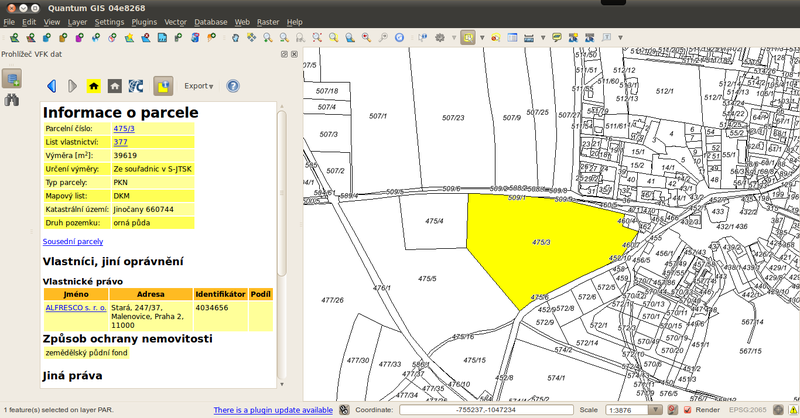
\includegraphics[height=5cm]{./pictures/Qgisvfkplugin.png}
      \caption{Ukázka prostředí pluginu (zdroj:
        %% ML: freegis.fsv.cvut.cz
        %% LK: opraveno
\href{http://freegis.fsv.cvut.cz/wiki/images/4/4b/Qgisvfkplugin-screenshot-05.png}{freegis.fsv.cvut.cz})}
      \label{fig:qgis_vfk_plugin}
  \end{figure}

Jde o zásuvný modul (anglicky plugin) pro geografický informační systém
%% ML: predlozka ``z'' neni v tomto kontextu moc vhodna
%% ML: predlozky mate v textu naduzivany a casto ve spatne kontextu (pod/z)
%% LK: na predlozky se zamerim 
QGIS, který umožňuje práci s daty českého katastru
%% ML: na tomto miste bych nepouzival ``uplne'', pro plugin je
%% podstatne, aby se v datech vyskytovali bloky PAR a BUD (skupina
%% NEMO), jinak nemusi byt '``uplna''
%% LK: odstraneno uplnymi, mám zmínit, že data musí obsahovat datovou skupinu NEMO?
%% ML: ano, muzete zminit
nemovitostí. Zásuvný modul pracuje s daty v takzvaném novém
výměnném formátu katastru, který je označovaný \zk{VFK} nebo
\zk{NVF}. Data ze souboru jsou čtena pomocí knihovny \zk{GDAL}. Plugin
%% ML: Pri cem jinem? ;-) Zkuste preformulovat
%% LK: preformulovano :)
%% ML: OK
umožňuje vyhledávání a zobrazování informací z načtených dat katastru
nemovitostí. Ovládání je uživatelsky přívětivé a známé vzhledem k
podobnému rozhraní jako je u webových aplikací.

%% ML: nyni?
%% LK: zmenen zacatek vety
%% ML: OK
V aktuální verzi je možné pro nahraná data vyhledávat: parcely, budovy, jednotky
a oprávněné osoby. Prohlížeč dat umožňuje zobrazit list vlastnictví a
další výpisy informací: o parcele, o budově, o jednotce a o oprávněné
osobě. Dále prohlížeč umožňuje zobrazení aktuálního stavu nemovitosti
na stránkách Nahlížení do katastru nemovitostí a export výpisů do
formátů HTML a zdrojového kódu LaTeXu (možnost vytvoření PDF a
PS\footnote{Programovací jazyk PostScript vyvinutý ke grafickému
  popisu tisknutelných dokumentů, výhodou je nezávislost na zařízení,
  ze kterého se tiskne, podobně jako formát PDF. \cite{PostScript}}).

%% ML: Obe vety zacinaji temer stejne: Zdrojove kody/texty, zkuste prepsat
%% ML: v poradku
Zdrojové kódy zásuvného modulu jsou ke stažení na adrese
\href{https://github.com/ctu-geoforall-lab/qgis-vfk-plugin}{Git
  repozitáře} a jsou šířeny pod licencí
\href{https://raw.githubusercontent.com/ctu-osgeorel/qgis-vfk-plugin/master/LICENSE}{GNU
  GPL}.

První verze zásuvného modulu (verze1.x) byla napsána v jazyce C++ a vyvinuta studenty
oboru Geoinformatika Annou Kratochvílovou a Václavem Petrášem na FSv
ČVUT v Praze v roce 2012. Druhá verze 2.x byla vyvíjena v letech 2015
a 2016 studentem stejného oboru Štěpánem Bambulou a zásuvný modul byl
přepsán do jazyka Python. \citep{vfk_qgis_plugin}
%http://freegis.fsv.cvut.cz/gwiki/VFK_/_QGIS_plugin
%https://cs.wikipedia.org/wiki/PostScript
 
\section{GDAL}
\label{sec:gdal}
\begin{figure}[H]
	 \centering
      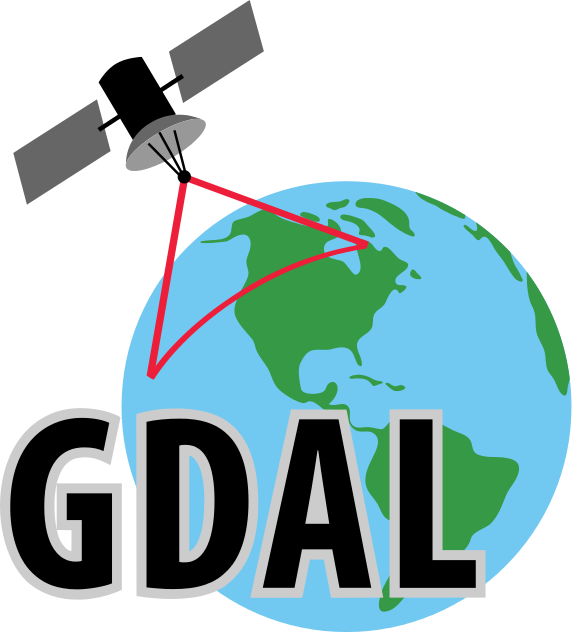
\includegraphics[height=5cm]{./pictures/gdal-logo.png}
      \caption{Logo GDAL (zdroj:
\href{https://upload.wikimedia.org/wikipedia/commons/thumb/d/df/GDALLogoColor.svg/572px-GDALLogoColor.svg.png}{gdal.org})}
      \label{fig:gdal}
  \end{figure}
  
Geospatial Data Abstraction Library (GDAL) je knihovna určená pro čtení
a zápis vektorových a rastrových formátů geodat. Jde o open source
vyvíjený pod licencí X/MIT a jako součást projektu Open Source
Geospatial Foundation (\zk{OSGeo}). Samotná knihovna je reprezentována
jedním abstraktním modelem pro rastrová data a jedním pro vektorová
data. Dále knihovna nabízí užitečné nástroje pro příkazovou řádku,
které slouží ke konverzi a zpracování dat. Od verze GDAL 2.0 je
součástí knihovny GDAL také knihovna OGR, která zajišťuje
funkcionalitu jednoduchých prvků vektorových dat.

Nejdříve byla knihovna vyvíjena Frankem Warmerdamem, od verze 1.3.2
došlo k převedení na GDAL/OGR Project Management Committee, který je
součástí \zk{OSGeo}. Knihovna je díky velké funkcionalitě často
využívána v komerční i nekomerční sféře a proto patří v \zk{GIS} mezi
hlavní volně dostupné softwary. \cite{gdal, gdal_wiki}
%obrazek: https://upload.wikimedia.org/wikipedia/commons/thumb/d/df/GDALLogoColor.svg/572px-GDALLogoColor.svg.png
%zdroje: http://www.gdal.org/, https://cs.wikipedia.org/wiki/GDAL

\section{Qt}

\begin{figure}[H]
	 \centering
      
\includegraphics[width=3cm]{./pictures/qt-logo.png}
      \caption{Logo Qt (zdroj:
\href{https://upload.wikimedia.org/wikipedia/commons/thumb/0/0b/Qt_logo_2016.svg/578px-Qt_logo_2016.svg.png}{wikipedia.org})}
      \label{fig:qt}
  \end{figure}

  %% ML: chybi Vam tu kontext: na tomto grafickem frameworku je postaven QGIS!
  %% ML: v poradku
  Qt je multiplatformní aplikační rámec (framework), který je určen
  pro vývoj aplikačního softwaru. Ten může snadno fungovat na různých
  platformách s žádnými nebo jen minimálními změnami v kódu. QGIS (viz
  kap. \ref{sec:qgis}) samotný je na tomto grafickém aplikačním rámci
  postaven. Qt je aktuálně vyvíjen společnostmi \textit{The Qt
    Company} a \textit{Qt Project}.\cite{qt_wiki, qt}

%zdroj: https://en.wikipedia.org/wiki/Qt_(software)
%obrazek: https://upload.wikimedia.org/wikipedia/commons/thumb/0/0b/Qt_logo_2016.svg/578px-Qt_logo_2016.svg.png

